\chapter{Groupe symétrique}

\minitoc

\begin{exo}
On pose \[\sigma_1=\begin{pmatrix}
1 & 2 & 3 & 4 & 5 \\
3 & 5 & 2 & 4 & 1
\end{pmatrix}\quad\sigma_2=\begin{pmatrix}
1 & 2 & 3 & 4 & 5 \\
2 & 1 & 5 & 4 & 3
\end{pmatrix}\quad\sigma_3=\begin{pmatrix}
1 & 2 & 3 & 4 & 5 & 6 & 7 \\
7 & 6 & 5 & 4 & 3 & 2 & 1
\end{pmatrix}\quad\sigma_4=\begin{pmatrix}
1 & 2 & 3 & 4 & 5 & 6 & 7 \\
5 & 4 & 6 & 3 & 7 & 2 & 1
\end{pmatrix}\]

Pour tout \(k\in\interventierii{1}{4}\) :

\begin{itemize}
\item Décomposer \(\sigma_k\) en produit de cycles à supports disjoints. \\

\item Calculer la signature de \(\sigma_k\). \\

\item Calculer \(\sigma_k^2\), \(\sigma_k\inv\) et \(\sigma_k^{2023}\).
\end{itemize}
\end{exo}

\begin{corr}
\note{À venir}
\end{corr}

\begin{exo}[Bon à retenir]
Soient \(n,k\in\N\) tels que \(2\leq k\leq n\).

Soient \(\sigma\in\S{n}\) et un \(k\)-cycle \[c=\begin{pmatrix}a_1 & a_2 & a_3 & \dots & a_k\end{pmatrix}\in\S{n}\] (avec \(a_1,\dots,a_k\in\interventierii{1}{n}\) deux à deux distincts).

Calculer \[\sigma c\sigma\inv.\]
\end{exo}

\begin{corr}
\note{À venir}
\end{corr}

\begin{exo}
Soit \(n\in\interventierie{2}{\pinf}\).

\begin{enumerate}
\item Montrer que si \(\tau,\tau\prim\in\S{n}\) sont des transpositions alors \[\quantifs{\exists\sigma\in\S{n}}\sigma\tau\sigma\inv=\tau\prim\] (on dit que les transpositions \(\tau\) et \(\tau\prim\) sont conjuguées dans \(\S{n}\)). \\

\item Quels sont les morphismes de groupes de \(\S{n}\) vers \(\accol{-1;1}\) ?
\end{enumerate}
\end{exo}

\begin{corr}
\note{À venir}
\end{corr}

\begin{exo}
Soient \(n\in\interventierie{3}{\pinf}\) et \(\sigma\in\S{n}\).

On suppose que \(\sigma\) commute avec toutes les permutations de \(\S{n}\).

Montrer \[\sigma=\id{}.\]
\end{exo}

\begin{corr}
\note{À venir}
\end{corr}

\begin{exo}
Soit \(n\in\interventierie{2}{\pinf}\).

On considère le \(n\)-cycle \[c=\begin{pmatrix}1 & 2 & 3 & \dots & n\end{pmatrix}\in\S{n}.\]

Quelles sont les permutations de \(\S{n}\) qui commutent avec \(c\) ?

On pourra identifier \(\interventierii{1}{n}\) avec \(\Z/n\Z\) de sorte que \[\quantifs{\forall x\in\Z/n\Z}c\paren{x}=x+1.\]
\end{exo}

\begin{corr}
\note{À venir}
\end{corr}

\begin{exo}
Soit \(n\in\Ns\).

Montrer que toute permutation \(\sigma\in\S{n}\) est produit de transpositions de la forme \(\begin{pmatrix}i & i+1\end{pmatrix}\) où \(i\in\interventierii{1}{n-1}\).
\end{exo}

\begin{corr}
\note{À venir}
\end{corr}

\begin{exo}[Groupe alterné \(\frakA{n}\)]
Soit \(n\in\Ns\).

\begin{enumerate}[series=exoAn]
\item Donner tous les éléments de \(\frakA{4}\) sous forme de produits de cycles à supports disjoints. \\

\item En supposant \(n\geq2\), quel est le cardinal de \(\frakA{n}\) ? \\

\item Donner une CNS sur \(n\) pour que le groupe \(\frakA{n}\) soit commutatif. \\

\item Montrer que tout élément de \(\frakA{n}\) est produit de \(3\)-cycles.
\end{enumerate}

On suppose désormais \(n\geq5\).

\begin{enumerate}[resume=exoAn]
\item Soient deux \(3\)-cycles \(c_1,c_2\in\frakA{n}\). Montrer \[\quantifs{\exists\sigma\in\frakA{n}}c_2=\sigma c_1\sigma\inv\] (on dit que \(c_1\) et \(c_2\) sont conjugués dans \(\frakA{n}\)). \\

\item Soient \(\groupe{G}[\times]\) un groupe abélien et \(\phi:\frakA{5}\to G\) un morphisme de groupes.

\begin{enumerate}
\item Montrer qu'il existe deux permutations \(a,b\in\frakA{5}\) telles que : \[\begin{dcases}a^3=\id{} \\ b^2=\id{} \\ \paren{ab}^5=\id{}\end{dcases}\]

\item Montrer \[a,b\in\ker\phi.\]

\textit{Indication :} utiliser le système et la commutativité de \(G\). \\

\item Montrer que \(\phi\) est constant. \\
\end{enumerate}

\item Montrer que tout morphisme de groupes de \(\frakA{n}\) vers un groupe abélien est constant\footnote{Cela montre que le groupe \(\frakA{n}\) n'est pas \guillemets{résoluble} si \(n\geq5\), proposition importante en \guillemets{théorie de Galois}. Cette démonstration provient de la belle conférence d'Alain Connes \guillemets{Évariste Galois et la théorie de l'ambiguïté} (on la trouve facilement sur internet).}.
\end{enumerate}
\end{exo}

\begin{corr}[1]
On a \[\begin{aligned}
\frakA{4}&=\left\lbrace\id{};\begin{pmatrix}1 & 2 & 3\end{pmatrix};\begin{pmatrix}3 & 2 & 1\end{pmatrix};\begin{pmatrix}1 & 2 & 4\end{pmatrix};\begin{pmatrix}4 & 2 & 1\end{pmatrix};\begin{pmatrix}1 & 3 & 4\end{pmatrix};\begin{pmatrix}4 & 3 & 1\end{pmatrix};\begin{pmatrix}2 & 3 & 4\end{pmatrix};\right. \\
&\color{white}=\lbrace\color{black}\left.\begin{pmatrix}4 & 3 & 2\end{pmatrix};\begin{pmatrix}1 & 2\end{pmatrix}\begin{pmatrix}3 & 4\end{pmatrix};\begin{pmatrix}1 & 3\end{pmatrix}\begin{pmatrix}2 & 4\end{pmatrix};\begin{pmatrix}1 & 4\end{pmatrix}\begin{pmatrix}2 & 3\end{pmatrix}\right\rbrace
\end{aligned}\]

On remarque \(\Card\frakA{4}=12\).
\end{corr}

\begin{corr}[2]
Montrons que \(\fonction{f}{\frakA{n}}{\S{n}\excluant\frakA{n}}{\sigma}{\begin{pmatrix}1 & 2\end{pmatrix}\sigma}\) est une bijection.

\(f\) est bien définie car \(\quantifs{\forall\sigma\in\frakA{n}}f\paren{\sigma}\in\S{n}\excluant\frakA{n}\).

Soit \(\sigma\prim\in\S{n}\excluant\frakA{n}\).

On a \[\begin{aligned}
\quantifs{\forall\sigma\in\frakA{n}}f\paren{\sigma}=\sigma\prim&\ssi\begin{pmatrix}1 & 2\end{pmatrix}\sigma=\sigma\prim \\
&\ssi\sigma=\begin{pmatrix}1 & 2\end{pmatrix}\sigma\prim.
\end{aligned}\]

De plus : \[\begin{aligned}
\epsilon\paren{\begin{pmatrix}1 & 2\end{pmatrix}\sigma\prim}&=\epsilon\paren{\begin{pmatrix}1 & 2\end{pmatrix}}\epsilon\paren{\sigma\prim} \\
&=\paren{-1}\paren{-1} \\
&=1.
\end{aligned}\]

Donc \(\begin{pmatrix}1 & 2\end{pmatrix}\sigma\prim\in\frakA{n}\).

Donc \(\begin{pmatrix}1 & 2\end{pmatrix}\sigma\prim\) est l'unique antécédent de \(\sigma\) par \(f\).

Donc \(f\) est une bijection.

Donc \(\Card\frakA{n}=\Card\paren{\S{n}\excluant\frakA{n}}\).

Or \(\S{n}=\frakA{n}\union\paren{\S{n}\excluant\frakA{n}}\) (réunion disjointe).

Donc \[\begin{aligned}
\Card\S{n}&=\Card\frakA{n}+\Card\paren{\S{n}\excluant\frakA{n}} \\
n!&=2\Card\frakA{n} \\
\dfrac{n!}{2}&=\Card\frakA{n}.
\end{aligned}\]
\end{corr}

\begin{corr}[3]
\(\frakA{1}\) et \(\frakA{2}\) sont clairement commutatifs.

De plus, \(\frakA{3}=\accol{\id{};\begin{pmatrix}1 & 2 & 3\end{pmatrix};\begin{pmatrix}3 & 2 & 1\end{pmatrix}}\) est commutatif car \(\begin{pmatrix}3 & 2 & 1\end{pmatrix}^2=\begin{pmatrix}1 & 2 & 3\end{pmatrix}\).

Enfin, dans \(\frakA{n}\) avec \(n\geq4\), on a \[\begin{dcases}
\begin{pmatrix}1 & 2 & 3\end{pmatrix}\begin{pmatrix}1 & 2 & 4\end{pmatrix}\paren{3}=1 \\
\begin{pmatrix}1 & 2 & 4\end{pmatrix}\begin{pmatrix}1 & 2 & 3\end{pmatrix}\paren{3}=2
\end{dcases}\] donc \(\begin{pmatrix}1 & 2 & 3\end{pmatrix}\) et \(\begin{pmatrix}1 & 2 & 4\end{pmatrix}\) ne commutent pas donc \(\frakA{n}\) n'est pas commutatif.

D'où la CNS : \[\frakA{n}\text{ est commutatif}\ssi n\leq3.\]
\end{corr}

\begin{corr}[4]
Soit \(\sigma\in\frakA{n}\).

Soient \(N\in\N\) et \(a_1,b_1,\dots,a_N,b_N\in\interventierii{1}{N}\) tels que \[\begin{dcases}\sigma=\begin{pmatrix}a_1 & b_1\end{pmatrix}\dots\begin{pmatrix}a_N & b_N\end{pmatrix} \\ \quantifs{\forall j\in\interventierii{1}{n}}a_j\not=b_j\end{dcases}\]

Comme \(\sigma\in\frakA{n}\), \(N\) est pair donc il existe \(k\in\N\) tel que \(N=2k\).

Donc \[\sigma=\underbrace{\begin{pmatrix}a_1 & b_1\end{pmatrix}\begin{pmatrix}a_2 & b_2\end{pmatrix}}_{\sigma_1}\dots\underbrace{\begin{pmatrix}a_{N-1} & b_{N-1}\end{pmatrix}\begin{pmatrix}a_N & b_N\end{pmatrix}}_{\sigma_k}.\]

Il suffit de montrer que \(\sigma_1,\dots,\sigma_k\) sont produits de \(3\)-cycles.

Montrons que \(\sigma_1\) est produit de \(3\)-cycles.

Si \(\Card\paren{\accol{a_1;b_1}\inter\accol{a_2;b_2}}=2\) alors \[\begin{pmatrix}a_1 & b_1\end{pmatrix}\begin{pmatrix}a_2 & b_2\end{pmatrix}=\id{}.\]

Si \(\Card\paren{\accol{a_1;b_1}\inter\accol{a_2;b_2}}=1\) : supposons par exemple \(b_1=a_2\). Alors \[\begin{pmatrix}a_1 & b_1\end{pmatrix}\begin{pmatrix}a_2 & b_2\end{pmatrix}=\begin{pmatrix}a_1 & b_1 & b_2\end{pmatrix}.\]

Si \(\Card\paren{\accol{a_1;b_1}\inter\accol{a_2;b_2}}=0\) alors \[\begin{aligned}
\begin{pmatrix}a_1 & b_1\end{pmatrix}\begin{pmatrix}a_2 & b_2\end{pmatrix}&=\begin{pmatrix}a_1 & b_1\end{pmatrix}\begin{pmatrix}b_1 & a_2\end{pmatrix}\begin{pmatrix}b_1 & a_2\end{pmatrix}\begin{pmatrix}a_2 & b_2\end{pmatrix} \\
&=\begin{pmatrix}a_1 & b_1 & a_2\end{pmatrix}\begin{pmatrix}b_1 & a_2 & b_2\end{pmatrix}.
\end{aligned}\]

Donc \(\sigma_1\) est produit de \(3\)-cycles.

De même, \(\quantifs{\forall i\in\interventierii{1}{k}}\sigma_k\text{ est produit de \(3\)-cycles}\).

Donc \(\sigma\) est produit de \(3\)-cycles.
\end{corr}

\begin{corr}[5]
Soient \(x_1,y_1,z_1,x_2,y_2,z_2\in\interventierii{1}{n}\) tels que \[\begin{dcases}c_1=\begin{pmatrix}x_1 & y_1 & z_1\end{pmatrix} \\ c_2=\begin{pmatrix}x_2 & y_2 & z_2\end{pmatrix}\end{dcases}\]

\(x_1,y_1,z_1\) sont deux à deux distincts et \(x_2,y_2,z_2\) aussi.

Soit \(\sigma\in\S{n}\) telle que \[\begin{dcases}\sigma\paren{x_1}=x_2 \\ \sigma\paren{y_1}=y_2 \\ \sigma\paren{z_1}=z_2\end{dcases}\]

On a \[\begin{aligned}
\sigma c_1\sigma\inv&=\begin{pmatrix}\sigma\paren{x_1} & \sigma\paren{y_1} & \sigma\paren{z_1}\end{pmatrix} \\
&=\begin{pmatrix}x_2 & y_2 & z_2\end{pmatrix} \\
&=c_2.
\end{aligned}\]

Soient \(a,b\in\interventierii{1}{n}\excluant\accol{x_1;y_1;z_1}\) tels que \(a\not=b\).

Posons \(\sigma\prim=\sigma\begin{pmatrix}a & b\end{pmatrix}\).

On a \[\begin{dcases}
\sigma\prim\paren{x_1}=x_2 \\
\sigma\prim\paren{y_1}=y_2 \\
\sigma\prim\paren{z_1}=z_2
\end{dcases}\]

Donc \(\sigma\prim c_1{\sigma\prim}\inv=c_2\).

On a \(\epsilon\paren{\sigma\prim}=-\epsilon\paren{\sigma}\).

Donc \(\sigma\) ou \(\sigma\prim\) est pair.

Donc \(c_1\) et \(c_2\) sont conjugués dans \(\frakA{n}\).
\end{corr}

\begin{corr}[6a]
On schématise la situation comme suit :

\begin{center}
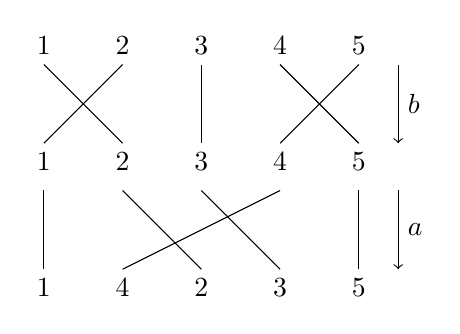
\begin{tikzpicture}
\draw (0,0) node[above] {\(1\)} -- (1,-1) node[below] {\(2\)};
\draw (1,0) node[above] {\(2\)} -- (0,-1) node[below] {\(1\)};
\draw (2,0) node[above] {\(3\)} -- (2,-1) node[below] {\(3\)};
\draw (3,0) node[above] {\(4\)} -- (4,-1) node[below] {\(5\)};
\draw (4,0) node[above] {\(5\)} -- (3,-1) node[below] {\(4\)};
\draw (0,-1.6) -- (0,-2.6) node[below] {\(1\)};
\draw (1,-1.6) -- (2,-2.6) node[below] {\(2\)};
\draw (2,-1.6) -- (3,-2.6) node[below] {\(3\)};
\draw (3,-1.6) -- (1,-2.6) node[below] {\(4\)};
\draw (4,-1.6) -- (4,-2.6) node[below] {\(5\)};
\draw[->] (4.5,0) -- (4.5,-1);
\draw[->] (4.5,-1.6) -- (4.5,-2.6);
\node[right] at (4.5,-0.5) {\(b\)};
\node[right] at (4.5,-2.1) {\(a\)};
\end{tikzpicture}
\end{center}

Prenons donc \(\begin{dcases}
a=\begin{pmatrix}2 & 3 & 4\end{pmatrix} \\
b=\begin{pmatrix}1 & 2\end{pmatrix}\begin{pmatrix}4 & 5\end{pmatrix}
\end{dcases}\)

On a bien \[\begin{dcases}
a^3=\id{} \\
b^2=\id{}
\end{dcases}\]

De plus, on a aussi \[\begin{aligned}
\paren{ab}^5&=\paren{\begin{pmatrix}2 & 3 & 4\end{pmatrix}\begin{pmatrix}1 & 2\end{pmatrix}\begin{pmatrix}4 & 5\end{pmatrix}}^5 \\
&=\begin{pmatrix}1 & 3 & 4 & 5 & 2\end{pmatrix}^5 \\
&=\id{}.
\end{aligned}\]
\end{corr}

\begin{corr}[6b]~\\
Posons \(\begin{dcases}
a\prim=\phi\paren{a} \\
b\prim=\phi\paren{b}
\end{dcases}\)

On a \({a\prim}^3=\phi\paren{a}^3=\phi\paren{a^3}=\phi\paren{\id{}}=1\).

De même, \({b\prim}^2=1\).

Donc \(\paren{a\prim b\prim}^5=1\).

De plus \(G\) est commutatif donc \(\paren{a\prim b\prim}^5={a\prim}^5{b\prim}^5\).

Donc \(1={a\prim}\inv b\prim\).

Donc \(a\prim=b\prim\).

Donc \({a\prim}^2=1\).

Donc \(a\prim={a\prim}^3{a\prim}^{-2}=1\).

Donc \(b\prim=1\).

Donc \(a,b\in\ker\phi\).
\end{corr}

\begin{corr}[6c]
Soit \(c\) un \(3\)-cycle.

Selon (5), il existe \(\sigma\in\frakA{n}\) telle que \(c=\sigma a\sigma\inv\) car \(a=\begin{pmatrix}2 & 3 & 4\end{pmatrix}\).

Donc \[\begin{WithArrows}
\phi\paren{c}&=\phi\paren{\sigma a\sigma\inv} \\
&=\phi\paren{\sigma}\phi\paren{a}\phi\paren{\sigma\inv} \Arrow{car \(G\) est commutatif} \\
&=\phi\paren{a}\phi\paren{\sigma}\phi\paren{\sigma\inv} \\
&=\phi\paren{a} \\
&=1.
\end{WithArrows}\]

Soit \(\sigma\prim\in\frakA{n}\).

Selon (4), \(\sigma\prim\) est produit de \(3\)-cycles.

Donc \(\phi\paren{\sigma\prim}=1\).
\end{corr}

\begin{corr}[7]
Soit \(\psi:\frakA{n}\to G\) un morphisme de groupes avec \(G\) abélien.

Posons \(\phi=\restr{\psi}{\frakA{5}}\).

Selon (6), \(\phi\) est constant.

Donc \[\psi\paren{\begin{pmatrix}1 & 2 & 3\end{pmatrix}}=\phi\paren{\begin{pmatrix}1 & 2 & 3\end{pmatrix}}=1.\]

Comme précédemment, on en déduit que tout \(3\)-cycle de \(\frakA{n}\) appartient à \(\ker\psi\) puis que \(\psi\) est constant.
\end{corr}